% !TEX root = ../beamer.tex

\begin{frame}[t]
	\frametitle{Model-Driven Software Development}
	\begin{center}
	\begin{tikzpicture}[
		>=stealth,
		box/.style = {draw, minimum width = 3cm, minimum height = 1.1cm, align=center},
		node distance = 1cm and 0.5cm
		]
		\node[box, fill=pantone315!10!white] (model) {Model};
		\node[box, below = of model] (dsl) {Domain-Specific\\Language};
		\draw[<-] (model) -- node[right] (uses) {} (dsl);
		\node[box, right = 1.75cm of uses] (generator) {Generator};
		\node[box, right = of generator] (platforms) {Code for\\Platforms};
		\draw[->] (dsl) -| (generator);
		\draw[->] (model) -| (generator);
		\draw[->] (generator) -- (platforms);
	\end{tikzpicture}
	\end{center}
	\vfill
    
    \begin{itemize}
       \item Cross-platform approach
       \item Develop a model once, for multiple platforms
       \item Development on a higher level of abstraction
    \end{itemize}
\end{frame}

%-----------------------------------------------------------------------------------

\begin{frame}
\frametitle{The \MD Framework}
	
	\begin{minipage}{.5\textwidth}
		\centering
		\begin{tikzpicture}
			\node[fill=white, draw, drop shadow] {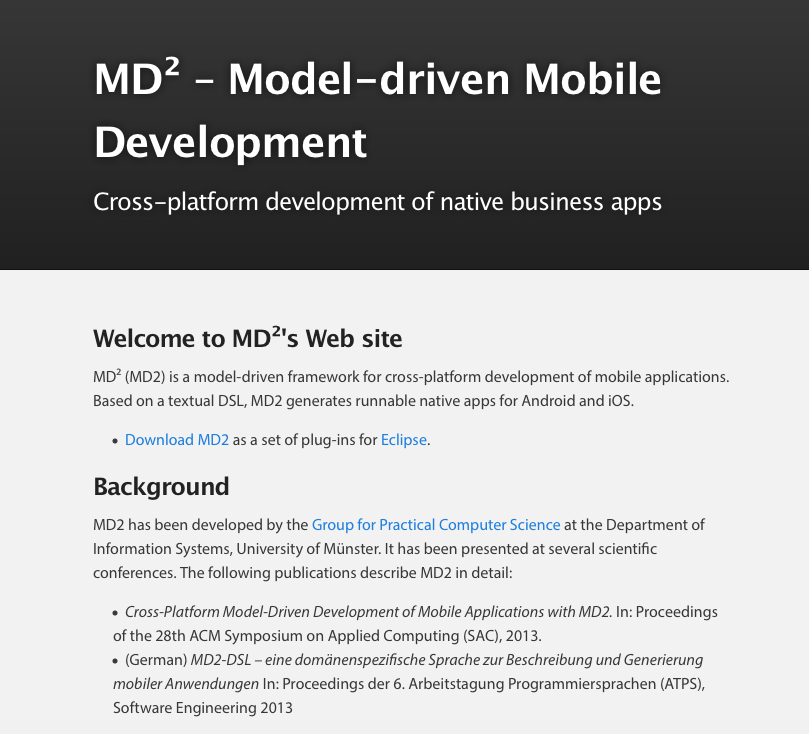
\includegraphics[width=\textwidth]{images/md2-web}};
		\end{tikzpicture}
		\quelle{\url{http://wwu-pi.github.io/md2-web/}}
	\end{minipage}\hfill
	\begin{minipage}{.45\textwidth}
		\begin{itemize}
			\item Cross-platform development of native business apps for mobile devices
			\item Developed by the Group for Practical Computer Science
			\item Open-source, available on Github
		\end{itemize}
	\end{minipage}
\end{frame}


\begin{frame}
    \frametitle{Starting Base of \MD}
    
    \begin{center}   
	    \begin{tikzpicture}[
		>=stealth,
		outer sep = 0pt,
		every node/.style={rectangle, draw, minimum height = 1.6em},
		bigbox/.style = {fill=gray!25!white, minimum width=7.5cm},
		smallbox/.style = {fill=gray!25!white, minimum width = 2.35cm},
		light/.style = {fill=gray!10!white},
		node distance = 0.2cm
		]
		{\small
			\node[bigbox] (md2model) {\MD Model};
			\node[light, below = 0cm of md2model.south west, anchor = north west, minimum width = 2.5cm] (model) {Model};
			\node[light, minimum width = 2.5cm, right = 0cm of model] (view) {View};
			\node[light, right = 0cm of view, minimum width = 2.5cm] (controller) {Controller};			
			\node[bigbox, below = of view] (preprocessing) {Preprocessing};			
			\draw[->] (view) -- (preprocessing);
		    
			\node[bigbox, below = of preprocessing] (completed) {Completed \MD Model};
			\draw[->] (preprocessing) -- (completed);
			
			\node[smallbox, below = of completed] (ios) {iOS\vphantom{Aq}};
			\node[smallbox, below = of completed.south west, anchor = north west] (android) {Android\vphantom{Aq}};
			\node[smallbox, below = of completed.south east, anchor = north east] (backend) {Backend\vphantom{Aq}};
			
			\draw[->] (completed) -- (ios.north);
			\draw[->] (completed) -- (android.north);
			\draw[->] (completed) -- (backend.north);
			
			\node[smallbox, below = of ios] (scios) {Source code};
			\node[smallbox, below = of android] (scandroid) {Source code};
			\node[smallbox, below = of backend] (scbackend) {Source code};
			
			\draw[->] (ios) -- (scios);
			\draw[->] (android) -- (scandroid);
			\draw[->] (backend) -- (scbackend);
			
			\node[smallbox, below = of scios] (iosapp) {iOS app\vphantom{Aq}};
			\node[smallbox, below = of scandroid] (androidapp) {Android app\vphantom{Aq}};
			\node[smallbox, below = of scbackend] (backendcontainer) {Container\vphantom{Aq}};
			
			\draw[->] (scios) -- (iosapp);
			\draw[->] (scandroid) -- (androidapp);
			\draw[->] (scbackend) -- (backendcontainer);
			
			\draw[thick, dashed, lightgray] ($ (android.north west) + (-0.1, 0.1) $) rectangle ($ (backend.south east) + (0.1, -0.1) $);
			\node[gray, overlay, left = 0.05cm of android, draw=none] {\tiny{Generator}};
		}
	    \end{tikzpicture}
    \end{center}
\hfill\quelle{Source: \MD Project Seminar Presentation}

\end{frame}

\begin{frame}
    \frametitle{\MD and \mapapps}
    
    \begin{center}   
	    \begin{tikzpicture}[
		>=stealth,
		outer sep = 0pt,
		every node/.style={rectangle, draw, minimum height = 1.6em},
		bigbox/.style = {fill=gray!25!white, minimum width=10cm},
		smallbox/.style = {fill=gray!25!white, minimum width = 2.35cm},
		new/.style = {fill=pantone315!10!white},
		light/.style = {fill=gray!10!white},
		unused/.style = {dotted, gray, fill=gray!5!white, text=lightgray},
		node distance = 0.2cm
		]
		{\small
			\node[bigbox] (md2model) {\MD Model};
			\node[light, below = 0cm of md2model.south west, anchor = north west, minimum width = 3.333333cm] (model) {Model};
			\node[light, minimum width = 3.333333cm, right = 0cm of model] (view) {View};
			\node[light, right = 0cm of view, minimum width = 3.333333cm] (controller) {Controller};
			
			\node[bigbox, below = of model.south west, anchor=north west] (preprocessing) {Preprocessing};			
			\draw[->] (view) -- (preprocessing);
		    
			\node[bigbox, below = of preprocessing] (completed) {Completed \MD Model};
			\draw[->] (preprocessing) -- (completed);
			
			\node[smallbox, unused, below = of completed.south west, anchor = north west] (android) {Android\vphantom{Aq}};
			\node[smallbox, unused, right = of android] (ios) {iOS\vphantom{Aq}};
			\node[smallbox, new, below = of completed.south east, anchor = north east] (mapapps) {map.apps\vphantom{Aq}};
			\node[smallbox, left = of mapapps] (backend) {Backend\vphantom{Aq}};
			
			\draw[->, lightgray] (completed) -- (ios.north);
			\draw[->, lightgray] (completed) -- (android.north);
			\draw[->] (completed) -- (backend.north);
			\draw[->] (completed) -- (mapapps.north);
			
			\node[smallbox, unused, below = of ios] (scios) {Source code};
			\node[smallbox, unused, below = of android] (scandroid) {Source code};
			\node[smallbox, below = of backend] (scbackend) {Source code};
			\node[smallbox, new, below = of mapapps] (scmapapps) {Source code};
			
			\draw[->, lightgray] (ios) -- (scios);
			\draw[->, lightgray] (android) -- (scandroid);
			\draw[->] (backend) -- (scbackend);
			\draw[->] (mapapps) -- (scmapapps);
			
			\node[smallbox, unused, below = of scios] (iosapp) {iOS app\vphantom{Aq}};
			\node[smallbox, unused, below = of scandroid] (androidapp) {Android app\vphantom{Aq}};
			\node[smallbox, below = of scbackend] (backendcontainer) {Container\vphantom{Aq}};
			\node[smallbox, new, below = of scmapapps] (mapappsapp) {map.apps app\vphantom{Aq}};
			
			\draw[->, lightgray] (scios) -- (iosapp);
			\draw[->, lightgray] (scandroid) -- (androidapp);
			\draw[->] (scbackend) -- (backendcontainer);
			\draw[->] (scmapapps) -- (mapappsapp);
			
			\draw[thick, dashed, lightgray] ($ (android.north west) + (-0.1, 0.1) $) rectangle ($ (mapapps.south east) + (0.1, -0.1) $);
			\node[gray, overlay, left = 0.05cm of android, draw=none] {\tiny{Generator}};
		}
	    \end{tikzpicture}
    \end{center}
	\hfill\quelle{Source: \MD Project Seminar Presentation}
\end{frame}

\begin{frame}[plain]
    \frametitle{Project Goals}
    
    \plainnumber
    
	\begin{center}
		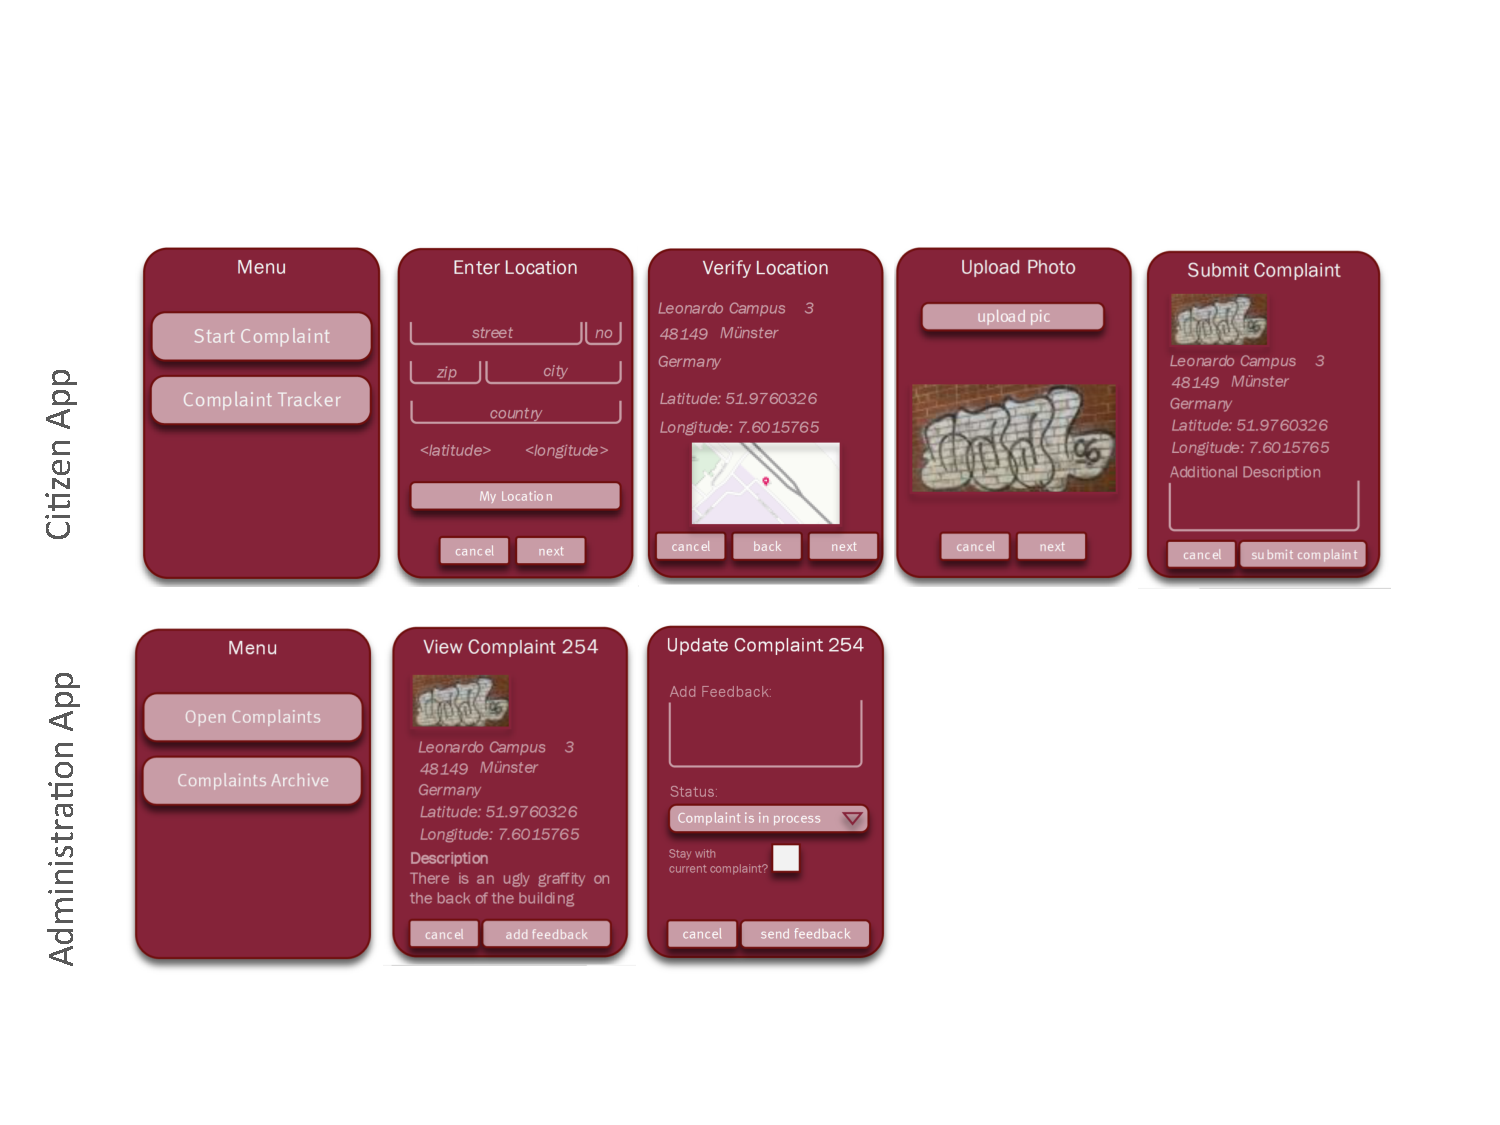
\includegraphics[width=.85\textwidth]{images/mockup}
	\end{center}
    
    \vspace{-1ex}
    
    \begin{itemize}
       \item Generate several apps from a single model
       \item Enable the specification of workflows across several apps
       \item The workflow specification should be simple, fast and easy to understand for both programmers and customers
       %\item Rough specification of a model should take no more than a few hours
    \end{itemize}
\end{frame}





